\pdfbookmark[0]{Front page}{label:frontpage}%

\begin{titlepage}
\newgeometry{top=0cm,bottom=1.2cm,right=0cm,left=0cm}

  \backgroundsetup{
   scale=1.1,
   angle=0,
   opacity=1.0,  %% adjust
   contents={\includegraphics[width=\paperwidth,height=\paperheight]{AAUgraphics/aau_waves}}
    }
		
  \begin{center} %%please do not change the height or width of the frontpage image
    \centerline{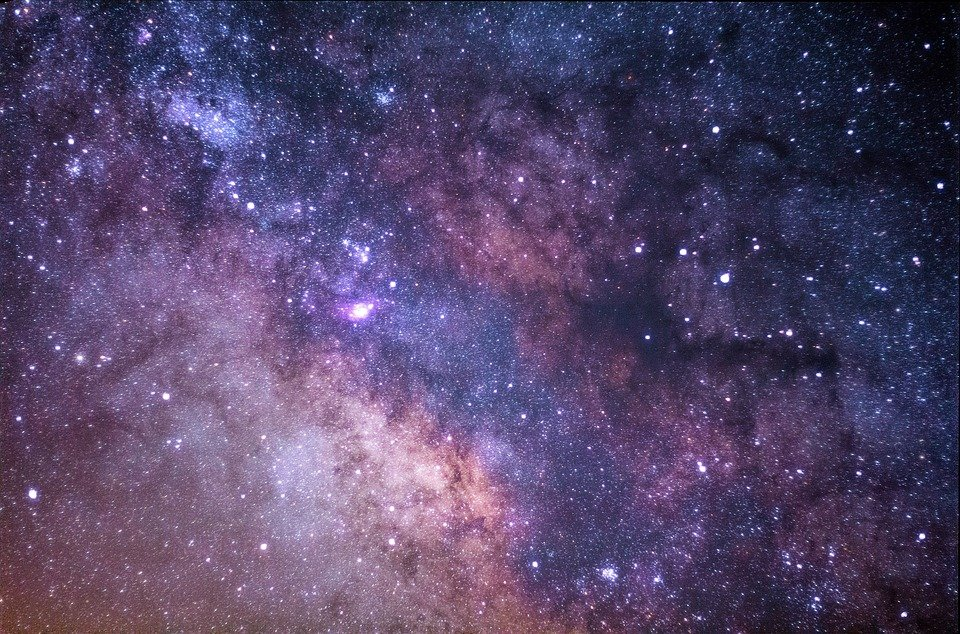
\includegraphics[totalheight=0.5\paperwidth,width=1\paperwidth]{AAUgraphics/frontpageImage}}% 
  \end{center}
	
	\vspace*{-0.96cm}
  {\noindent\color{aaublue}\fboxsep0pt\colorbox{white}{\begin{tabular}{@{}p{\paperwidth}@{}}
    \centerline{
    \begin{minipage}{0.85\textwidth}
        \bigskip
				\bigskip
        \centering
        \Huge{\textbf{
Internship at CERN % insert your title here
        }}
    \end{minipage}
    }
		
	\centerline{
	\begin{minipage}{0.9\textwidth}
        \bigskip
        \centering
        \Large{
Development of the EMP % insert your subtitle here
        }
    \end{minipage}
    }
			
	\centerline{
	\begin{minipage}{0.9\textwidth}
        \bigskip
        \centering
        {\Large
Emil Hammer Sandgaard% insert names separated by comma
        }
    \end{minipage}
    }
			
    \centerline{
    \begin{minipage}{0.9\textwidth}
        \bigskip
        \centering
        {\large
Electronic Engineering \the\year-06% insert name of study, group number, year-month
        } 
    \end{minipage}
    }
			
    \centerline{
    \begin{minipage}{0.9\textwidth}
        \bigskip
        \centering
%% Comment this section if you are not doing Bachelor or Master Project   
        {\Large
6. semester
      %Bachelor Project
        }
        \smallskip
    \end{minipage}
    }
			
  \end{tabular}}}

  \vfill
  \begin{figure}[!b]
	\centering
    
\includegraphics[width=0.2\paperwidth]{AAUgraphics/aau_logo_circle_en}% comment this line in for English version
    %\includegraphics[width=0.2\paperwidth]{AAUgraphics/aau_logo_circle_da} %comment this line in for Danish version
  \end{figure}
\end{titlepage}
\restoregeometry